\chapter{Manutenção}
\label{cap-manutencao}

A manutenção pode ser considerada a atividade que mais passou por mudanças nos últimos anos. Isso é resultado da complexidade e diversidade das tarefas que devem ser realizadas pelos seus responsáveis. O aumento na diversidade de equipamentos eletrônicos que dão suporte a atividades corriqueiras e essências, e devem ser mantidos, é um dos grandes desafios que deve ser encarado pelas empresas e organizações.

Equipamentos eletrônicos estão presentes em todos os momentos do cotidiano de um empresa, seja um computador, uma televisão, um projetor, entre outros. Como mantê-los de forma que eles sejam nossos aliados e não nossos inimigos? A resposta está em evoluir a manutenção junto com a quantidade e diversidade dos ativos da sua empresa.
	
Um trecho da introdução do livro de Kardec e Nascif, Manutenção - Função Estratégica, chama atenção por descrever exatamente a mudança primordial exigida no setor de manutenção, se o para paradigma anterior, e ainda atual na maioria das empresas, era: "O homem de manutenção sente-se bem quando executa um bom reparo", o novo paradigma é: "O homem de manutenção sente-se bem  quando não tem que fazer reparo porque conseguiu evitar todas as quebras não planejadas".
	
A manutenção irá extrapolar o seu próprio significado, que de acordo com o BSI \cite{british1993bs} é "A combinação de todas as ações técnicas e administrativas associadas destinadas a reter um item ou restaurá-lo em um estado no qual possa desempenhar sua função requerida". Manutenção será atrelada a inovação e não apenas a preservarção do estado de um ativo. É preciso pensar em como evitar e prever, o mau funcionamento, parada ou até perda de um ativo.
	
Como então alinhar a manutenção aos objetivos da organização, fazendo dela uma ferramenta poderosa de preservação e aumento do tempo de vida dos ativos da organização, resultando na diminuição de custos com consertos on demand, atividades paradas, entre outros. Este capítulo apresentará tipos de manutenções disponíveis, sobre gerenciamento de manutenção e suas aplicações.


\section{Tipos de Manutenção}


Kardec e Nascif citam seis tipos de manutenção, mostrados na Figura~\ref{tiposmanutencao}, que de forma geral englobam os tantos outros existentes. A Figura, resumi estes dtipos e como eles se relacionam.

\graphicspath{{figuras/}}
\begin{figure}[h]
\centering
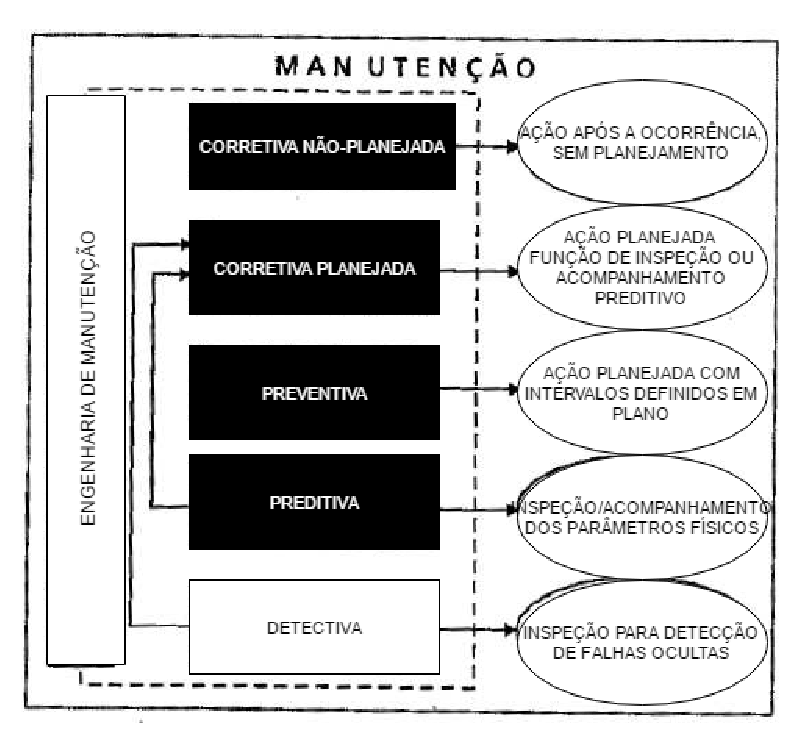
\includegraphics[width=0.8\textwidth]{tipos-de-manutencao}
\caption{Tipos de Manutenção \textbf{Fonte: Manutenção - Função Estratégica, 2009, pg. 38}}
\label{tiposmanutencao}
\end{figure}




\begin{enumerate}
	\item \textbf{Manutenção Corretiva}

		\emph{"Manutenção Corretiva é a atuação para a correção da falha ou do desempenho menor do que esperado."} \cite{kardecnascif2010}

		\emph{"Manutenção realizada após uma falha destinada a colocar um item em um estado onde possa executar uma função necessária de forma segura e eficiente"} \cite{british1993bs}

		Ocorre em equipamentos com defeito ou que estão funcionando de forma diferentedo esperado. Sua principal ação é Corrigir ou Restaurar para o estado de funcionamento. Pode ser Planejada ou Não Planejada.

		\begin{itemize}
			\item \textbf{Manutenção Corretiva Não Planejada:} configura na correção da falha realizada de forma aleatória, após a o fato já ocorrido. Acarreta em custos altos, com a própria ação da correção, perda de qualidade do equipamento, interrupção das atividades onde o equipamento é necessário.
			\item \textbf{Manutenção Corretiva Planejada:} configura na correção da falha realizada de forma aleatória, após a o fato já ocorrido. Acarreta em custos altos, com a própria ação da correção, perda de qualidade do equipamento, interrupção das atividades onde o equipamento é necessário.
		\end{itemize}

		\graphicspath{{figuras/}}
		\begin{figure}[h]
		\centering
		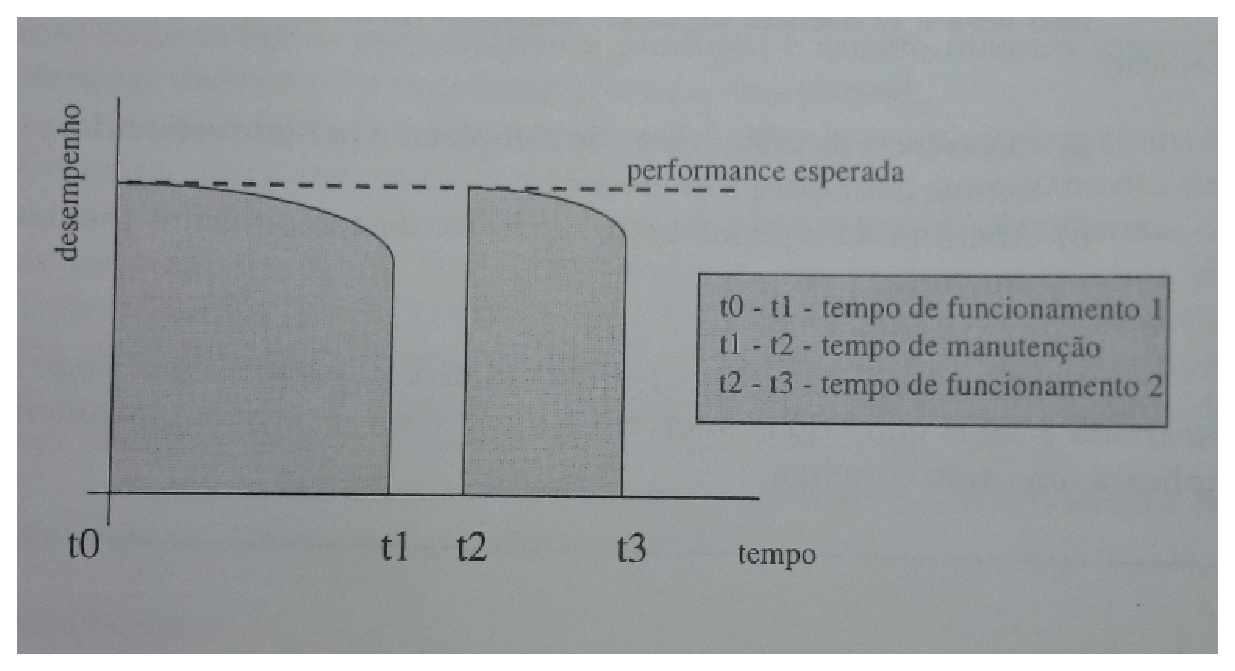
\includegraphics[width=0.8\textwidth]{corretiva}
		\caption{Manutenção Corretiva \textbf{Fonte: Manutenção - Função Estratégica, 1998, pg. 35}}
		\label{corretiva}
		\end{figure}

	\item \textbf{Manutenção Preventiva}

		\emph{"Manutenção Preventiva é a atuação realizada de forma a reduzir ou evitar a falha ou queda no desempenho, obedecendo a um plano previamente elaborado, baseado em intervalos definidos de tempo."} \cite{kardecnascif2010}

		A manutenção preventiva busca evitar a ocorrência de falhas. Sua adoção é mais adequada quando a reposição de equipamentos for simples, tiver custo alto de falhas e as falhas forem mais prejudiciais as atividades.

		\graphicspath{{figuras/}}
		\begin{figure}[h]
		\centering
		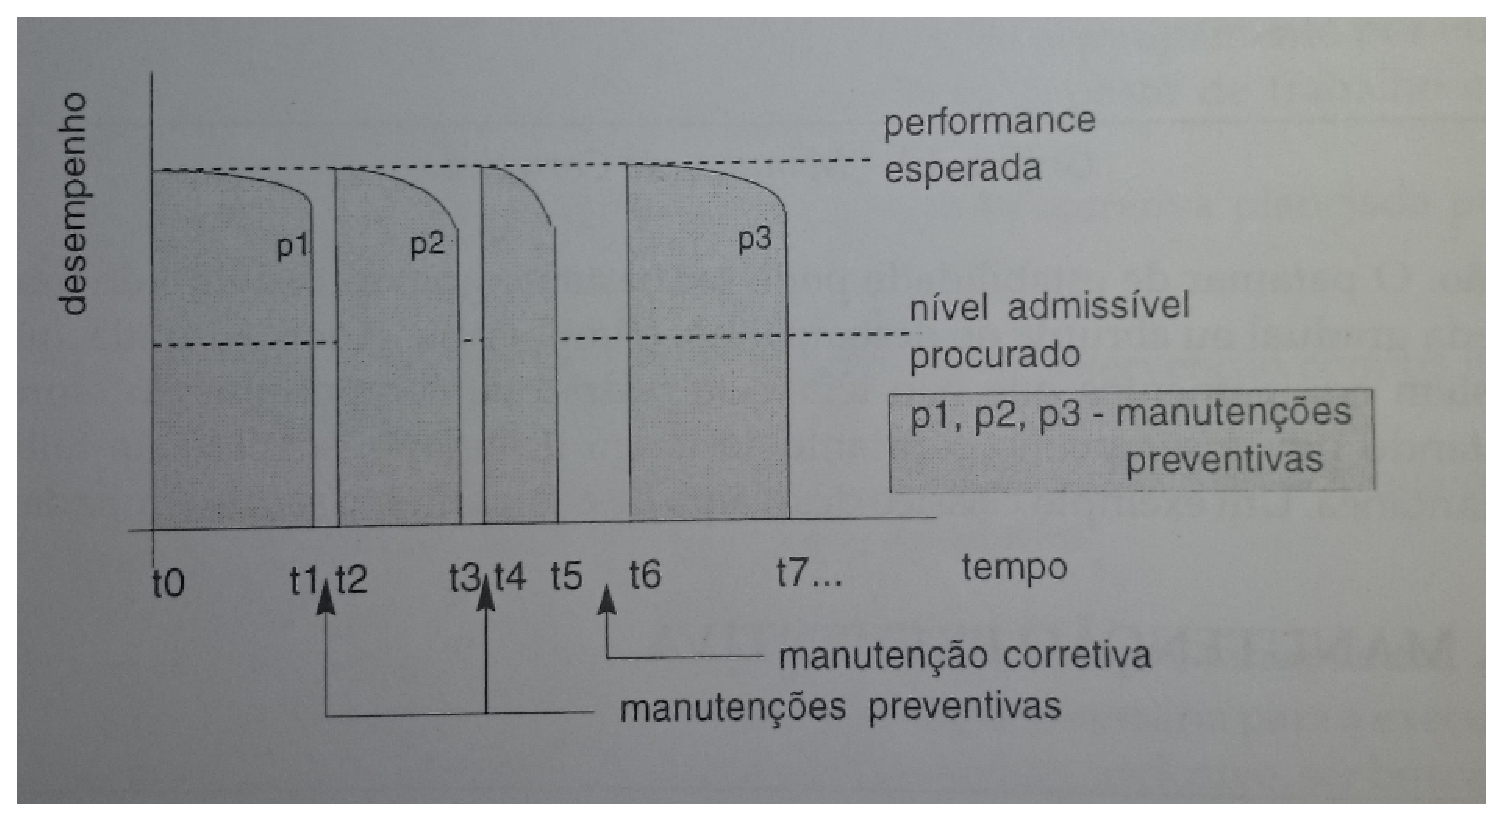
\includegraphics[width=0.8\textwidth]{preventiva}
		\caption{Manutenção Preventiva \textbf{Fonte: Manutenção - Função Estratégica, 1998, pg. 36}}
		\label{preventiva}
		\end{figure}


	\item \textbf{Manutenção Preditiva}

		\emph{"Manutenção Preditiva é a atuação realizada com base em modificações de parâmetros de condição ou desempenho, cujo acompanhamento obedece a uma sistemática."} \cite{kardecnascif2010}

		Visa a operação do contínua do equipamento por mais tempo possível, as medições e verificações são realizadas com o equipamento em produção, ou seja, com ele funcionando e operando na suas atividades. 

		Segundo Kardec e Nascif, indica-se na adoção da manutenção preditiva a análise dos fatores abaixo:

			\begin{itemize}
				\item Aspectos relacionados com a segurança pessoal e operacional.
				\item Redução de custos pelo acompanhamento constante das condições dos equipamentos, evitando assim intervenções desnecessárias.
				\item Manter os equipamentos operando, de modo seguro, por mas tempo.
			\end{itemize}

		\graphicspath{{figuras/}}
		\begin{figure}[h]
		\centering
		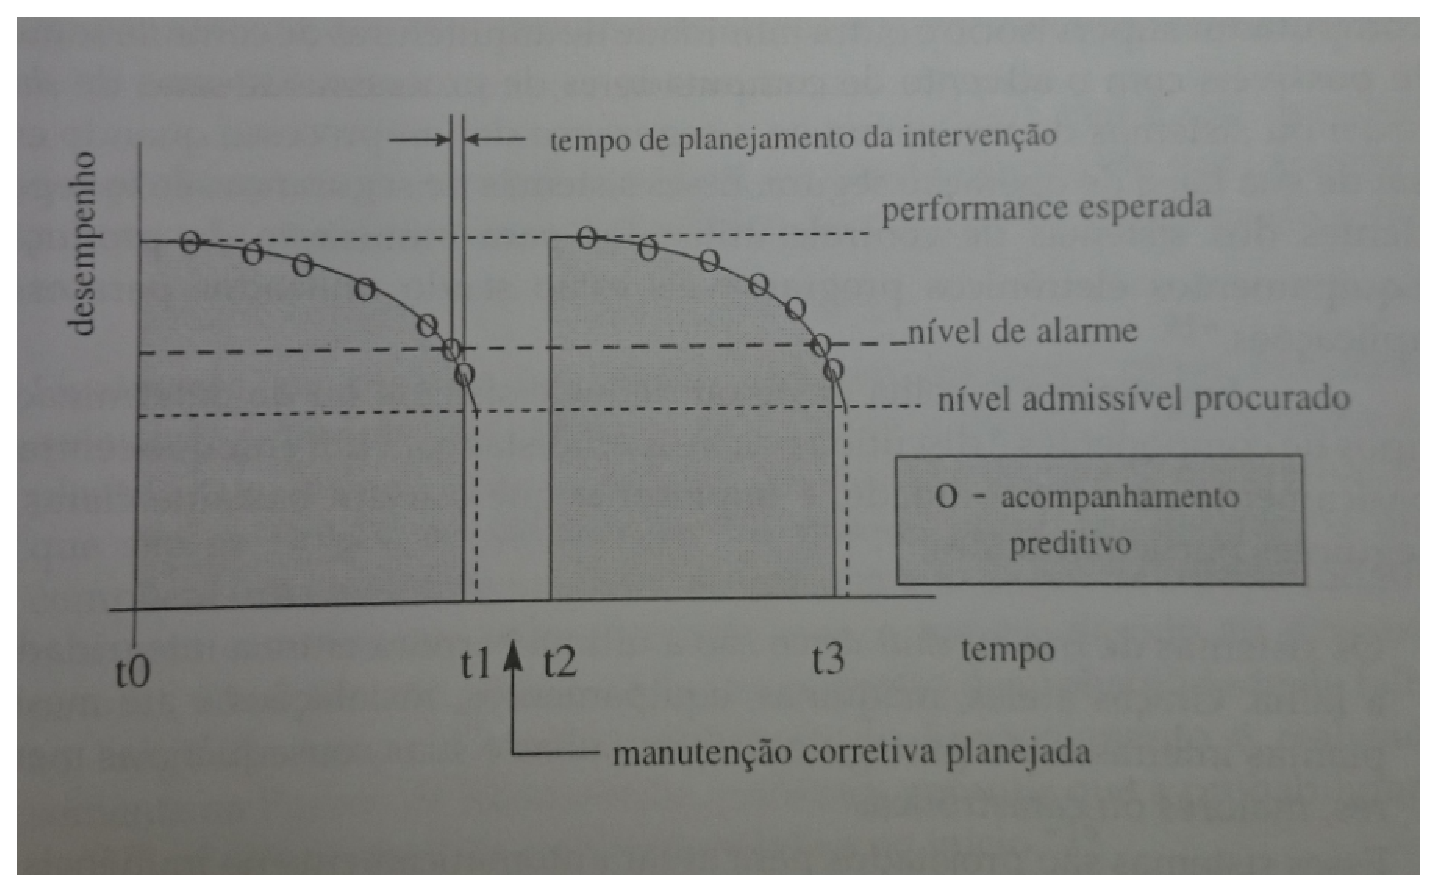
\includegraphics[width=0.8\textwidth]{preditiva}
		\caption{Manutenção Preditiva \textbf{Fonte: Manutenção - Função Estratégica, 1998, pg. 37}}
		\label{preditiva}
		\end{figure}
		

	\item \textbf{Manutenção Detectiva}

		\emph{"Manutenção Detectiva é a atuação efetuada em sistemas de proteção buscando detectar falhas ocultas ou não perceptíveis ao pessoal de operação e manutenção."} \cite{kardecnascif2010}

		Detectar falhas ocultas é fundamental para garantir a confiabilidade, os especialistas verificam o sistema sem tirá-lo de operação, detectam falhas ocultas e podem corrigir a situação, com o sistema operando.


\end{enumerate}



\textbf{PARTE ANTIGA}


A European Federation of National Maintenance Societies (EFNMS) define manutenção como a combinação de toda ação técnica, administrativa e gerencial que, durante o ciclo de vida de um ativo, tenha a intenção de mantê-lo ou restaurá-lo para o estado útil, realizando a função requerida. Diz, ainda, que a manutenção tem importância máxima para o negócio e o comércio, bem como para o meio ambiente e, em geral, para a saúde e a segurança \cite{efnms}.

\section{Tipos de Manutenção}

Existem diferentes tipos de manutenção e eles são distintos e dependentes do contexto, da natureza da tarefa em que serão aplicados. Araújo \cite{araujo2015} traz a definição de quatro tipos de manutenção, sendo elas:

\begin{enumerate}
	\item \textbf{Manutenção Corretiva:} é a intervenção quando ocorre uma falha, sendo que essa falha torna o equipamento indisponível ou com baixa confiabilidade, isso não significa que ela seja uma manutenção de emergência, pois existem duas classes de manutenção corretiva.
		\begin{enumerate}
			\item \textbf{manutenção corretiva não planejada:} nela a intervenção é imediata, sem tempo para preparação do serviço.
			\item \textbf{manutenção corretiva planejada:} nela a intervenção no equipamento é programada. Pode-se optar pela operação do equipamento até ele quebrar, depende da decisão gerencial.
		\end{enumerate}
	\item \textbf{Manutenção Preventiva:} nesse tipo realiza-se a manutenção como objetivo de reduzir ou evitar a falha ou queda de desempenho do equipamento, seguindo um plano previamente elaborado, e são realizadas periodicamente. Ela procura evitar a ocorrência de falhas, por meio do conhecimento prévio de ações que devem ser tomadas.
	\item \textbf{Manutenção Preditiva:} consiste na modificação de um parâmetro de condição ou desempenho, seu acompanhamento segue uma sistemática. Utiliza instrumentos de manutenção, para prevenir falhas em equipamentos ou sistemas por meio de parâmetros diversos, que irão permitir a operação contínua do equipamento pelo máximo tempo possível.
	\item \textbf{Manutenção proativa:} tem como base a frequência na ocorrência da falha. É feito um histórico dessas ocorrências no equipamento e retiradas informações para saber qual a causa básica de falhas frequentes. Ela gera ações que está relacionadas a causa raíz da falha, com o objetivo de aumentar o tempo de vida do equipamento.
\end{enumerate}

Esses quatro tipos mostram conceitos diferentes, mas também muito próximos, trazendo uma certa dificuldade em pensar qual seria melhor para um determinado contexto a ser trabalhado. Muitas vezes eles podem se tornar complementares. Garrido \cite{garrido} ainda diz que é muito difícil encontrar uma aplicação para cada conceito, e que por isso, muitas vezes é mais valoroso usar mais de um tipo ao contexto sendo trabalhado. Por isso ele traz a ideia de Modelos de Manutenção, que misturam os tipos acima citados e assim podem atender as necessidades de manutenção de um certo tipo de equipamento.

\section{Modelos de Manutenção}
\label{sec_modelos_manutencao}

A seguir serão explicados os modelos de manutenção definidos por Garrido.

\begin{enumerate}
	\item \textbf{Modelo Corretivo:} consiste no modelo mais básico, sendo aplicado em equipamentos com menor criticidade no seu uso, ou seja, seu uso não compromete fatalmente a tarefa à qual ele dá suporte. Os defeitos encontrados não são um problema econômico ou técnico. 
	\item \textbf{Modelo Condicional:} utiliza as atividades do modelo corretivo, acrescentando uma série de testes que irão definir uma ação seguinte. Caso encontre-se algo errado nos testes realizados, é agendada uma intervenção. Esse modelo é aplicável em equipamentos pouco utilizados ou cujo a probabilidade de falha é pequena.
	\item \textbf{Modelo Sistemático:} consiste em executar um conjunto de atividades, medições e experimentos independente do estado equipamento, para então reparar falhas que poderão surgir. É utilizado em equipamentos de média disponibilidade e nível de importância no sistema, onde sua falha possa trazer algum tipo de problema. Um exemplo de uso seria um reator descontínuo. 
	\item \textbf{Modelo de Manutenção de Alta Disponibilidade:} é o modelo mais exaustivo, por ser aplicado em equipamentos que necessitem de uma disponibilidade acima de 90\%, esse tipo de equipamento gera altos custos na produção caso ocorra uma falha nele, pois caso ele tenha que ficar parado, pode comprometer as atividades que ele executa. Por isso não existe tempo para parar o equipamento, como exige os outros modelos citados. Assim são utilizadas técnicas da manutenção preditiva, para conhecer o estado do equipamento e também realizar manutenções programadas, com revisões completas, com um frequência anual ou superior, que tem o intuito de substituir peças sujeitas a desgastes ou com maior probabilidade de falhas. 
	\\
	Este modelo também traz a necessidade de se realizar manutenções corretivas e reparações provisórias, que manterão o equipamento funcionando até a próxima revisão. Exemplos de uso deste modelo: Fornos de alta temperatura e depósitos de reatores.
\end{enumerate} 

Além de modelos que podem ser criados por cada organização, de acordo com a necessidade e o tipo de equipamentos existentes, também pode se criar classificações para os tipos de equipamentos, sistemas ou componentes. No exemplo utilizado por \cite{valeria2013}, foram utilizados três tipos de classificações para esses itens, sendo elas:

\begin{itemize}
	\item críticos: podem parar as atividades ou causar danos;
	\item não críticos: apresentam histórico de alto custo operacional, ou de reparo, ou substituição, podem demandar longo tempo para aquisição ou são considerados obsoletos;
	\item podem funcionar até falhar.
\end{itemize}

Classificar os elementos ou criar modelos de manutenção, são formas de se facilitar o controle sobre os ativos e saber suas características e o papel que exercem no negócio.

\subsection{Origem dos danos}

É fato que todos componentes das máquinas, equipamentos e instalações, bem como os prédios e as benfeitorias inevitavelmente se desgastem ao longo tempo, necessitando assim de um conjunto de tratativas e cuidados técnic

os periódicos para se manterem em condições de pleno funcionamento, devido a isso a manutenção, hoje vista como área estratégica, assume uma importância fundamental da gestão dos ativos, com reflexos diretos nos nível de operação, logística, Disponibilidadeidade e confiabilidade dos meios produtivos. Consoante ao escopo deste trabalho entenda-se aqui ativos como os equipamentos eletroeletrônicos, todavia muitos dos princípios e conhecimentos aqui abordados são úteis a gestão eficiente de todos os demais ativos de uma organização. 

São múltiplas as causas que levam a deterioração e ao desgaste dos ativos de uma organização, podendo ter natureza mecânica, elétrica, térmica, química ou operacional, sendo na maioria das vezes uma associação destas. Segundo Seeling \cite{seeling2000} as causas corriqueiras que merecem destaque são:

\begin{itemize}
	\item o atrito entre peças móveis em operação;
	\item os esforços realizados pelos componentes em funcionamento normal;
	\item os esforços estáticos e dinâmicos suportados pelas estruturas;
	\item o calor, frio, umidade;
	\item a pressão, vibração, oxidação (ferrugem);
	\item a sujeira acumulada, abrasão;
	\item a corrosão pelo ataque químico dos elementos existentes no ambiente;
	\item as intempéries que agem sobre os materiais expostos ao tempo.
\end{itemize}


A consequência cumulativa das fontes de desgaste, descritas acima, são os defeitos e as falhas. Sendo o defeito definido como a situação que não impede o funcionamento do equipamento, todavia pode acarretar a curto ou longo prazo a sua indisponibilidade, já a falha é descrita como as ocorrências que impedem o equipamento ou instalação de funcionar tornando-o indisponível, ou seja, é quando deixamos de executar certas tarefas, porque no momento em que o equipamento foi solicitado, ele falhou. Por esta razão, e tendo em vista que as falhas nos equipamentos podem representar grandes perdas para a imagem das organizações, a redução e o controle destas fontes de desgaste e deterioração são essenciais.

As raízes das falhas de um equipamento estão nos danos sofridos pelas suas peças ou componentes, pois normalmente um equipamento não quebra totalmente de uma vez, mas para de funcionar quando alguma parte primária de seu conjunto se danifica. A parte primária avariada pode estar dentro do hardware, em um componente ou ao longo de um circuito em diversos pontos, por exemplo, a fonte é uma parte vital para que um circuito funcione, assim como suas trilhas para a passagem de corrente elétrica.

Sendo assim, antes de pensar em manutenção e seus indicadores de performace que tanto podem contribuir para a melhoria da gestão dos ativos, as empresas e organizações públicas precisam conhecer em quais condições irão fazer uso de seus equipamentos, e quais são suas condições ideais de operação, pois precisam adotar ações adequadas e com o menor custo. Esta compreensão a auxiliará na tomada de decisão em dois momentos, no momento da aquisição e no do uso produtivo desses equipamentos, pois não é inteligente, nem economicamente atrativo fazer uso de equipamentos em condições diferentes das quais foi planejado, pois por muitas vezes pode ser observado, para equipamentos eletrônicos, que o custo médio de manutenção, ao longo de sua vida útil pode ser muito superior ao custo de aquisição do próprio equipamento. Entenda-se tempo de vida útil a fase de utilização do ciclo de vida do ativo, ou seja, é o período de tempo iniciado no momento de sua aquisição (entrada em operação), com duração estimada de tempo (meses ou anos) que possa cumprir corretamente a função técnica para o qual foi concebido, durante o qual o mesmo realiza um trabalho com rentabilidade. 

Muitas são as considerações a serem feitas no momento da escolha de um equipamento eletroeletrônico, sendo algumas delas a disponibilidade de peças de reposição, qualidade, confiabilidade, manutenabilidade, dimensões físicas, infra-estrutura necessária, prazo de entrega, preço e treinamentos necessários para instalação, operação e manutenção. 

Do ponto de vista da organização, a melhor escolha é a que apresenta o menor custo de ciclo de vida (utilização) do ativo, e o maior tempo de operação sem manutenção. Isto é, os menores custos envolvidos na aquisição de equipamentos para testes, manutenção e partes de reposição (inclusive um equipamento completo), bem como o custo envolvido com a parada do equipamento no período da manutenção.
